% !TEX encoding = UTF-8 Unicode
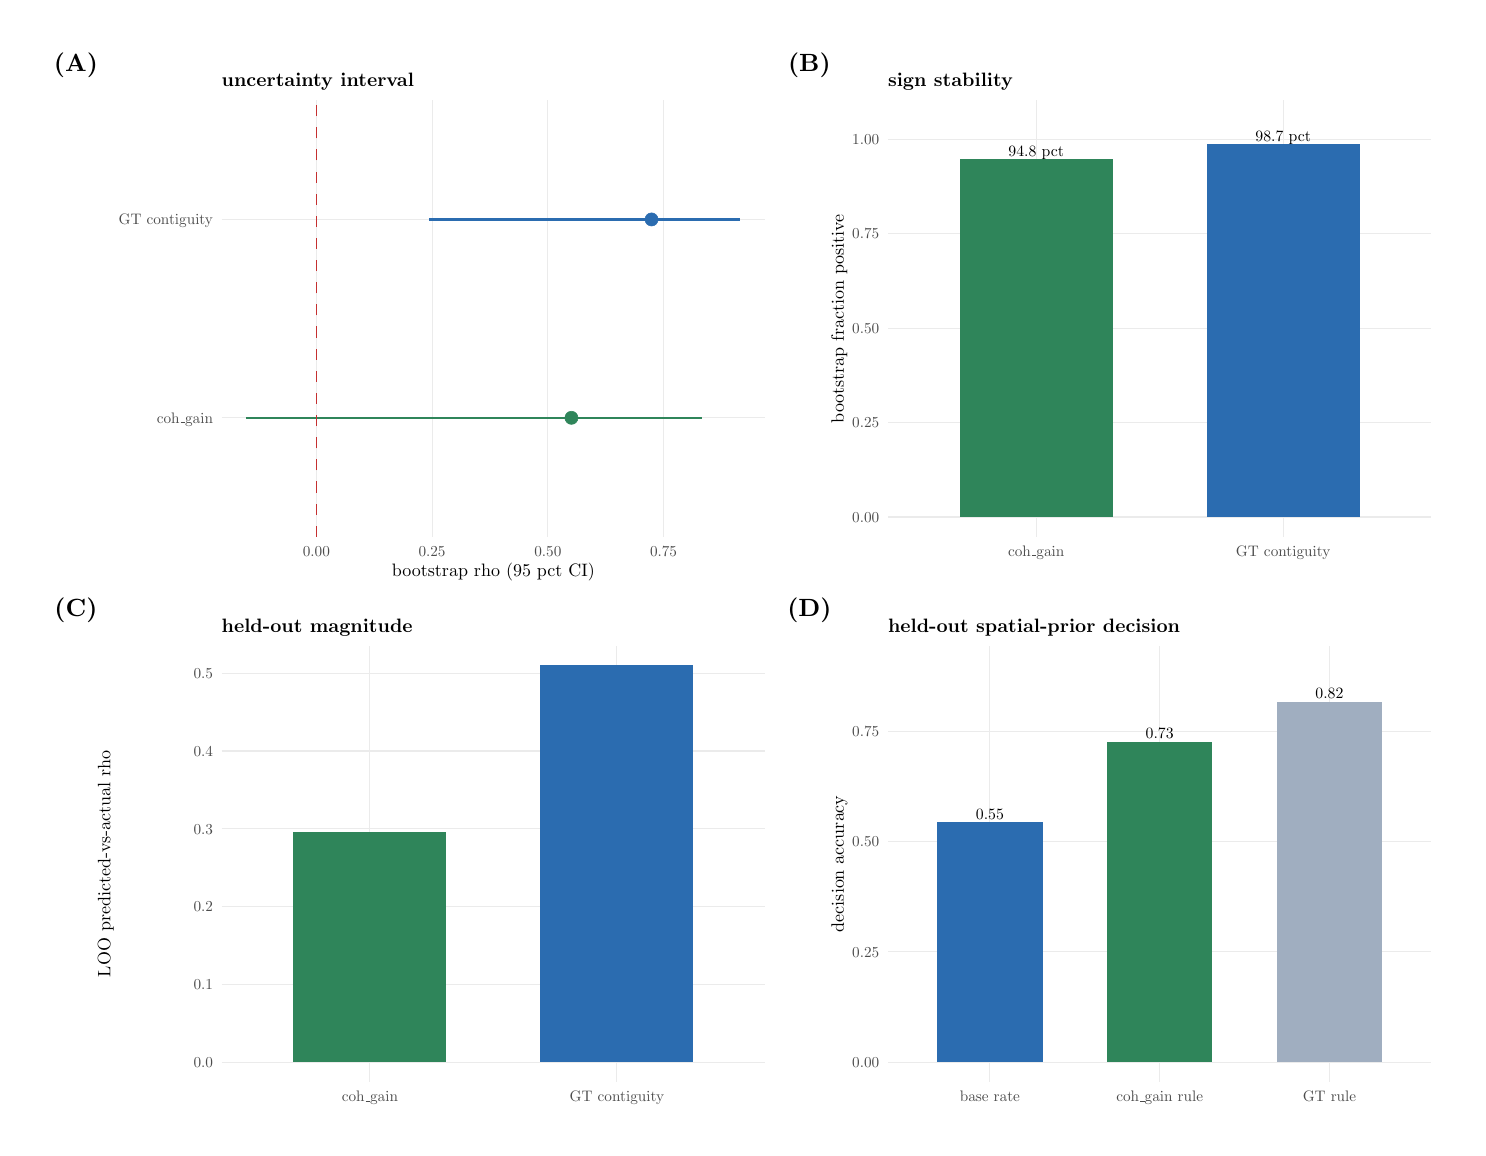
\begin{tikzpicture}[x=1pt,y=1pt]
\definecolor{fillColor}{RGB}{255,255,255}
\path[use as bounding box,fill=fillColor,fill opacity=0.00] (0,0) rectangle (516.73,397.48);
\begin{scope}
\path[clip] (  0.00,  0.00) rectangle (516.73,397.48);
\definecolor{drawColor}{RGB}{255,255,255}
\definecolor{fillColor}{RGB}{255,255,255}

\path[draw=drawColor,line width= 0.6pt,line join=round,line cap=round,fill=fillColor] (  0.00,  0.00) rectangle (516.73,397.48);
\end{scope}
\begin{scope}
\path[clip] (  5.50,195.00) rectangle (270.47,391.98);
\definecolor{fillColor}{RGB}{255,255,255}

\path[fill=fillColor] (  5.50,195.00) rectangle (270.47,391.99);
\end{scope}
\begin{scope}
\path[clip] (270.47,195.00) rectangle (511.23,391.98);
\definecolor{fillColor}{RGB}{255,255,255}

\path[fill=fillColor] (270.47,195.00) rectangle (511.23,391.99);
\end{scope}
\begin{scope}
\path[clip] (  5.50,  5.50) rectangle (270.47,195.00);
\definecolor{fillColor}{RGB}{255,255,255}

\path[fill=fillColor] (  5.50,  5.50) rectangle (270.47,195.00);
\end{scope}
\begin{scope}
\path[clip] (270.47,  5.50) rectangle (511.23,195.00);
\definecolor{fillColor}{RGB}{255,255,255}

\path[fill=fillColor] (270.47,  5.50) rectangle (511.23,195.00);
\end{scope}
\begin{scope}
\path[clip] ( 70.12,213.50) rectangle (266.47,371.19);
\definecolor{drawColor}{gray}{0.92}

\path[draw=drawColor,line width= 0.4pt,line join=round] ( 70.12,256.50) --
	(266.47,256.50);

\path[draw=drawColor,line width= 0.4pt,line join=round] ( 70.12,328.18) --
	(266.47,328.18);

\path[draw=drawColor,line width= 0.4pt,line join=round] (104.31,213.50) --
	(104.31,371.19);

\path[draw=drawColor,line width= 0.4pt,line join=round] (146.13,213.50) --
	(146.13,371.19);

\path[draw=drawColor,line width= 0.4pt,line join=round] (187.96,213.50) --
	(187.96,371.19);

\path[draw=drawColor,line width= 0.4pt,line join=round] (229.78,213.50) --
	(229.78,371.19);
\definecolor{drawColor}{RGB}{43,108,176}

\path[draw=drawColor,line width= 0.8pt,line join=round] (144.96,328.18) -- (257.55,328.18);
\definecolor{drawColor}{RGB}{47,133,90}

\path[draw=drawColor,line width= 0.8pt,line join=round] ( 79.05,256.50) -- (243.66,256.50);
\definecolor{drawColor}{RGB}{43,108,176}
\definecolor{fillColor}{RGB}{43,108,176}

\path[draw=drawColor,line width= 0.2pt,line join=round,line cap=round,fill=fillColor] (225.43,328.18) circle (  2.37);
\definecolor{drawColor}{RGB}{47,133,90}
\definecolor{fillColor}{RGB}{47,133,90}

\path[draw=drawColor,line width= 0.2pt,line join=round,line cap=round,fill=fillColor] (196.49,256.50) circle (  2.37);
\definecolor{drawColor}{RGB}{197,48,48}

\path[draw=drawColor,line width= 0.4pt,dash pattern=on 4pt off 4pt ,line join=round] (104.31,213.50) -- (104.31,371.19);
\end{scope}
\begin{scope}
\path[clip] (  0.00,  0.00) rectangle (516.73,397.48);
\definecolor{drawColor}{gray}{0.30}

\node[text=drawColor,anchor=base east,inner sep=0pt, outer sep=0pt, scale=  0.55] at ( 66.97,254.61) {coh{\_{}}gain};

\node[text=drawColor,anchor=base east,inner sep=0pt, outer sep=0pt, scale=  0.55] at ( 66.97,326.29) {GT contiguity};
\end{scope}
\begin{scope}
\path[clip] (  0.00,  0.00) rectangle (516.73,397.48);
\definecolor{drawColor}{gray}{0.30}

\node[text=drawColor,anchor=base,inner sep=0pt, outer sep=0pt, scale=  0.55] at (104.31,206.56) {0.00};

\node[text=drawColor,anchor=base,inner sep=0pt, outer sep=0pt, scale=  0.55] at (146.13,206.56) {0.25};

\node[text=drawColor,anchor=base,inner sep=0pt, outer sep=0pt, scale=  0.55] at (187.96,206.56) {0.50};

\node[text=drawColor,anchor=base,inner sep=0pt, outer sep=0pt, scale=  0.55] at (229.78,206.56) {0.75};
\end{scope}
\begin{scope}
\path[clip] (  0.00,  0.00) rectangle (516.73,397.48);
\definecolor{drawColor}{RGB}{0,0,0}

\node[text=drawColor,anchor=base,inner sep=0pt, outer sep=0pt, scale=  0.65] at (168.30,199.26) {bootstrap rho (95 pct CI)};
\end{scope}
\begin{scope}
\path[clip] (  0.00,  0.00) rectangle (516.73,397.48);
\definecolor{drawColor}{RGB}{0,0,0}

\node[text=drawColor,anchor=base west,inner sep=0pt, outer sep=0pt, scale=  0.70] at ( 70.12,376.05) {\bfseries uncertainty interval};
\end{scope}
\begin{scope}
\path[clip] (  0.00,  0.00) rectangle (516.73,397.48);
\definecolor{drawColor}{RGB}{0,0,0}

\node[text=drawColor,anchor=base,inner sep=0pt, outer sep=0pt, scale=  0.90] at ( 17.44,381.82) {\bfseries (A)};
\end{scope}
\begin{scope}
\path[clip] (310.88,213.50) rectangle (507.23,371.19);
\definecolor{drawColor}{gray}{0.92}

\path[draw=drawColor,line width= 0.4pt,line join=round] (310.88,220.66) --
	(507.23,220.66);

\path[draw=drawColor,line width= 0.4pt,line join=round] (310.88,254.80) --
	(507.23,254.80);

\path[draw=drawColor,line width= 0.4pt,line join=round] (310.88,288.93) --
	(507.23,288.93);

\path[draw=drawColor,line width= 0.4pt,line join=round] (310.88,323.06) --
	(507.23,323.06);

\path[draw=drawColor,line width= 0.4pt,line join=round] (310.88,357.19) --
	(507.23,357.19);

\path[draw=drawColor,line width= 0.4pt,line join=round] (364.43,213.50) --
	(364.43,371.19);

\path[draw=drawColor,line width= 0.4pt,line join=round] (453.68,213.50) --
	(453.68,371.19);
\definecolor{fillColor}{RGB}{43,108,176}

\path[fill=fillColor] (426.01,220.66) rectangle (481.35,355.42);
\definecolor{fillColor}{RGB}{47,133,90}

\path[fill=fillColor] (336.76,220.66) rectangle (392.10,350.10);
\definecolor{drawColor}{RGB}{0,0,0}

\node[text=drawColor,anchor=base,inner sep=0pt, outer sep=0pt, scale=  0.57] at (453.68,356.40) {98.7 pct};

\node[text=drawColor,anchor=base,inner sep=0pt, outer sep=0pt, scale=  0.57] at (364.43,351.08) {94.8 pct};
\end{scope}
\begin{scope}
\path[clip] (  0.00,  0.00) rectangle (516.73,397.48);
\definecolor{drawColor}{gray}{0.30}

\node[text=drawColor,anchor=base east,inner sep=0pt, outer sep=0pt, scale=  0.55] at (307.73,218.77) {0.00};

\node[text=drawColor,anchor=base east,inner sep=0pt, outer sep=0pt, scale=  0.55] at (307.73,252.90) {0.25};

\node[text=drawColor,anchor=base east,inner sep=0pt, outer sep=0pt, scale=  0.55] at (307.73,287.04) {0.50};

\node[text=drawColor,anchor=base east,inner sep=0pt, outer sep=0pt, scale=  0.55] at (307.73,321.17) {0.75};

\node[text=drawColor,anchor=base east,inner sep=0pt, outer sep=0pt, scale=  0.55] at (307.73,355.30) {1.00};
\end{scope}
\begin{scope}
\path[clip] (  0.00,  0.00) rectangle (516.73,397.48);
\definecolor{drawColor}{gray}{0.30}

\node[text=drawColor,anchor=base,inner sep=0pt, outer sep=0pt, scale=  0.55] at (364.43,206.56) {coh{\_{}}gain};

\node[text=drawColor,anchor=base,inner sep=0pt, outer sep=0pt, scale=  0.55] at (453.68,206.56) {GT contiguity};
\end{scope}
\begin{scope}
\path[clip] (  0.00,  0.00) rectangle (516.73,397.48);
\definecolor{drawColor}{RGB}{0,0,0}

\node[text=drawColor,rotate= 90.00,anchor=base,inner sep=0pt, outer sep=0pt, scale=  0.65] at (294.94,292.34) {bootstrap fraction positive};
\end{scope}
\begin{scope}
\path[clip] (  0.00,  0.00) rectangle (516.73,397.48);
\definecolor{drawColor}{RGB}{0,0,0}

\node[text=drawColor,anchor=base west,inner sep=0pt, outer sep=0pt, scale=  0.70] at (310.88,376.05) {\bfseries sign stability};
\end{scope}
\begin{scope}
\path[clip] (  0.00,  0.00) rectangle (516.73,397.48);
\definecolor{drawColor}{RGB}{0,0,0}

\node[text=drawColor,anchor=base,inner sep=0pt, outer sep=0pt, scale=  0.90] at (282.47,381.82) {\bfseries (B)};
\end{scope}
\begin{scope}
\path[clip] ( 70.12, 16.51) rectangle (266.47,174.20);
\definecolor{drawColor}{gray}{0.92}

\path[draw=drawColor,line width= 0.4pt,line join=round] ( 70.12, 23.68) --
	(266.47, 23.68);

\path[draw=drawColor,line width= 0.4pt,line join=round] ( 70.12, 51.79) --
	(266.47, 51.79);

\path[draw=drawColor,line width= 0.4pt,line join=round] ( 70.12, 79.89) --
	(266.47, 79.89);

\path[draw=drawColor,line width= 0.4pt,line join=round] ( 70.12,108.00) --
	(266.47,108.00);

\path[draw=drawColor,line width= 0.4pt,line join=round] ( 70.12,136.11) --
	(266.47,136.11);

\path[draw=drawColor,line width= 0.4pt,line join=round] ( 70.12,164.22) --
	(266.47,164.22);

\path[draw=drawColor,line width= 0.4pt,line join=round] (123.67, 16.51) --
	(123.67,174.20);

\path[draw=drawColor,line width= 0.4pt,line join=round] (212.92, 16.51) --
	(212.92,174.20);
\definecolor{fillColor}{RGB}{43,108,176}

\path[fill=fillColor] (185.26, 23.68) rectangle (240.59,167.03);
\definecolor{fillColor}{RGB}{47,133,90}

\path[fill=fillColor] ( 96.01, 23.68) rectangle (151.34,106.88);
\end{scope}
\begin{scope}
\path[clip] (  0.00,  0.00) rectangle (516.73,397.48);
\definecolor{drawColor}{gray}{0.30}

\node[text=drawColor,anchor=base east,inner sep=0pt, outer sep=0pt, scale=  0.55] at ( 66.97, 21.78) {0.0};

\node[text=drawColor,anchor=base east,inner sep=0pt, outer sep=0pt, scale=  0.55] at ( 66.97, 49.89) {0.1};

\node[text=drawColor,anchor=base east,inner sep=0pt, outer sep=0pt, scale=  0.55] at ( 66.97, 78.00) {0.2};

\node[text=drawColor,anchor=base east,inner sep=0pt, outer sep=0pt, scale=  0.55] at ( 66.97,106.11) {0.3};

\node[text=drawColor,anchor=base east,inner sep=0pt, outer sep=0pt, scale=  0.55] at ( 66.97,134.22) {0.4};

\node[text=drawColor,anchor=base east,inner sep=0pt, outer sep=0pt, scale=  0.55] at ( 66.97,162.33) {0.5};
\end{scope}
\begin{scope}
\path[clip] (  0.00,  0.00) rectangle (516.73,397.48);
\definecolor{drawColor}{gray}{0.30}

\node[text=drawColor,anchor=base,inner sep=0pt, outer sep=0pt, scale=  0.55] at (123.67,  9.57) {coh{\_{}}gain};

\node[text=drawColor,anchor=base,inner sep=0pt, outer sep=0pt, scale=  0.55] at (212.92,  9.57) {GT contiguity};
\end{scope}
\begin{scope}
\path[clip] (  0.00,  0.00) rectangle (516.73,397.48);
\definecolor{drawColor}{RGB}{0,0,0}

\node[text=drawColor,rotate= 90.00,anchor=base,inner sep=0pt, outer sep=0pt, scale=  0.65] at ( 29.85, 95.35) {LOO predicted-vs-actual rho};
\end{scope}
\begin{scope}
\path[clip] (  0.00,  0.00) rectangle (516.73,397.48);
\definecolor{drawColor}{RGB}{0,0,0}

\node[text=drawColor,anchor=base west,inner sep=0pt, outer sep=0pt, scale=  0.70] at ( 70.12,179.06) {\bfseries held-out magnitude};
\end{scope}
\begin{scope}
\path[clip] (  0.00,  0.00) rectangle (516.73,397.48);
\definecolor{drawColor}{RGB}{0,0,0}

\node[text=drawColor,anchor=base,inner sep=0pt, outer sep=0pt, scale=  0.90] at ( 17.44,184.83) {\bfseries (C)};
\end{scope}
\begin{scope}
\path[clip] (310.88, 16.51) rectangle (507.23,174.20);
\definecolor{drawColor}{gray}{0.92}

\path[draw=drawColor,line width= 0.4pt,line join=round] (310.88, 23.68) --
	(507.23, 23.68);

\path[draw=drawColor,line width= 0.4pt,line join=round] (310.88, 63.50) --
	(507.23, 63.50);

\path[draw=drawColor,line width= 0.4pt,line join=round] (310.88,103.32) --
	(507.23,103.32);

\path[draw=drawColor,line width= 0.4pt,line join=round] (310.88,143.14) --
	(507.23,143.14);

\path[draw=drawColor,line width= 0.4pt,line join=round] (347.70, 16.51) --
	(347.70,174.20);

\path[draw=drawColor,line width= 0.4pt,line join=round] (409.06, 16.51) --
	(409.06,174.20);

\path[draw=drawColor,line width= 0.4pt,line join=round] (470.41, 16.51) --
	(470.41,174.20);
\definecolor{fillColor}{RGB}{160,174,192}

\path[fill=fillColor] (451.39, 23.68) rectangle (489.44,153.97);
\definecolor{fillColor}{RGB}{47,133,90}

\path[fill=fillColor] (390.03, 23.68) rectangle (428.08,139.48);
\definecolor{fillColor}{RGB}{43,108,176}

\path[fill=fillColor] (328.67, 23.68) rectangle (366.72,110.49);
\definecolor{drawColor}{RGB}{0,0,0}

\node[text=drawColor,anchor=base,inner sep=0pt, outer sep=0pt, scale=  0.57] at (470.41,154.95) {0.82};

\node[text=drawColor,anchor=base,inner sep=0pt, outer sep=0pt, scale=  0.57] at (409.06,140.46) {0.73};

\node[text=drawColor,anchor=base,inner sep=0pt, outer sep=0pt, scale=  0.57] at (347.70,111.47) {0.55};
\end{scope}
\begin{scope}
\path[clip] (  0.00,  0.00) rectangle (516.73,397.48);
\definecolor{drawColor}{gray}{0.30}

\node[text=drawColor,anchor=base east,inner sep=0pt, outer sep=0pt, scale=  0.55] at (307.73, 21.78) {0.00};

\node[text=drawColor,anchor=base east,inner sep=0pt, outer sep=0pt, scale=  0.55] at (307.73, 61.60) {0.25};

\node[text=drawColor,anchor=base east,inner sep=0pt, outer sep=0pt, scale=  0.55] at (307.73,101.42) {0.50};

\node[text=drawColor,anchor=base east,inner sep=0pt, outer sep=0pt, scale=  0.55] at (307.73,141.25) {0.75};
\end{scope}
\begin{scope}
\path[clip] (  0.00,  0.00) rectangle (516.73,397.48);
\definecolor{drawColor}{gray}{0.30}

\node[text=drawColor,anchor=base,inner sep=0pt, outer sep=0pt, scale=  0.55] at (347.70,  9.57) {base rate};

\node[text=drawColor,anchor=base,inner sep=0pt, outer sep=0pt, scale=  0.55] at (409.06,  9.57) {coh{\_{}}gain rule};

\node[text=drawColor,anchor=base,inner sep=0pt, outer sep=0pt, scale=  0.55] at (470.41,  9.57) {GT rule};
\end{scope}
\begin{scope}
\path[clip] (  0.00,  0.00) rectangle (516.73,397.48);
\definecolor{drawColor}{RGB}{0,0,0}

\node[text=drawColor,rotate= 90.00,anchor=base,inner sep=0pt, outer sep=0pt, scale=  0.65] at (294.94, 95.35) {decision accuracy};
\end{scope}
\begin{scope}
\path[clip] (  0.00,  0.00) rectangle (516.73,397.48);
\definecolor{drawColor}{RGB}{0,0,0}

\node[text=drawColor,anchor=base west,inner sep=0pt, outer sep=0pt, scale=  0.70] at (310.88,179.06) {\bfseries held-out spatial-prior decision};
\end{scope}
\begin{scope}
\path[clip] (  0.00,  0.00) rectangle (516.73,397.48);
\definecolor{drawColor}{RGB}{0,0,0}

\node[text=drawColor,anchor=base,inner sep=0pt, outer sep=0pt, scale=  0.90] at (282.47,184.83) {\bfseries (D)};
\end{scope}
\end{tikzpicture}
